\documentclass[12pt]{article}
\usepackage[utf8]{inputenc}
\usepackage{graphics}
\usepackage[english,russian]{babel}
\usepackage{graphicx}
\usepackage{longtable}
\usepackage[left=25mm, top=20mm, right=25mm, bottom=30mm,nohead,nofoot]{geometry}
\usepackage{verbatim}

\setcounter{tocdepth}{4}

\begin{document}

\begin{titlepage}
	\center
		Санкт-Петербургский Политехнический 
		университет Петра Великого
		Институт прикладной математики и механики
		\\ \textbf{Кафедра «Прикладная математика»}

	\vfill ~
	\textbf{
		\\ \large ЛАБОРАТОРНАЯ РАБОТА №1
		\\	\normalsize	
			Сравнение распределений выборок для различных 
		\\	функций распределения с теоретическими оценками
	}
	\\	по дисциплине 
	\\	"Математическая статистика"

	\vfill ~

	Выполнил студент гр. \textbf{33631/1} \\
	\textbf{Лансков.Н.В.} \\ 

\vfill

{\large}	Санкт-Петербург
\\ 2019
\end{titlepage}

%%%
% Table of conetnts 
%%%
% \settocdepth{chapter}
\tableofcontents
\pagebreak

% \setcounter{chapter}{1}

%%%
% Text
%%%
\section{Постановка задачи}
Сравнить графики распределения выборок случайных чисел, сгенерированных при помощи различных функций распределения, с теоретическими кривыми распределения для выборок мощностями 10, 50, 100.

\section{Теория}
Рассмотрим использованные распределения подробней.

\subsection{Нормальное распределение}

\begin{equation} \label{eq1}
f(x)= \frac{1}{\sigma\sqrt{2\pi}}e^{-\frac{(x - x_0)^2}{2\sigma^2}}
\end{equation}

\subsection{Распределение Коши}

\begin{equation} \label{eq2}
f(x)= \frac{1}{\pi}\bigg[ \frac{\gamma}{(x - x_0)^2 + \gamma^2}\ \bigg]
\end{equation}

\subsection{Распределение Лапласа}

\begin{equation} \label{eq3}
f(x)= \frac{\alpha}{2}e^{-\alpha|x - \beta|}
\end{equation}

\subsection{Равномерное распределение}

\begin{equation} \label{eq4}
f(x)= \frac{1}{b - a}
\end{equation}

\subsection{Распределение Пуассона}

\begin{equation} \label{eq5}
P(\lambda) = \frac{\lambda^k}{k!}e^{-\lambda}
\end{equation}

\pagebreak

\section{Реализация}
Выполнено средствами \textit{python} c применением библиотек \textit{numpy, scipy and matplotlib}

\section{Результаты}

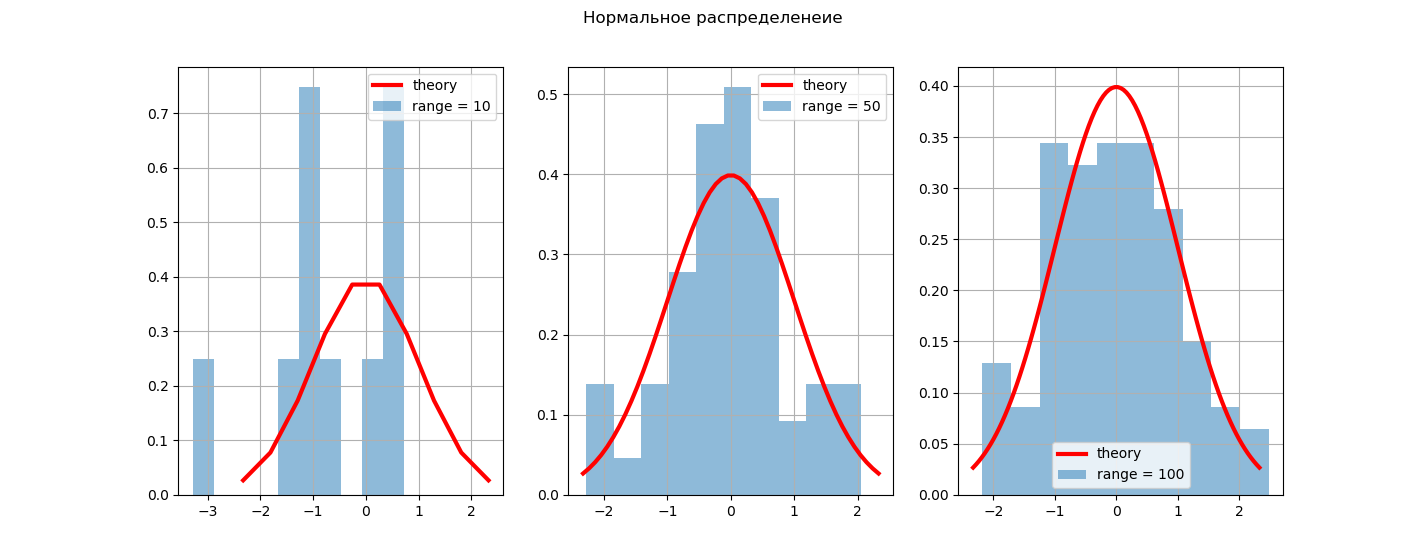
\includegraphics[width=\textwidth]{normal.png}
\begin{center}
Рис. 1. 
\end{center}

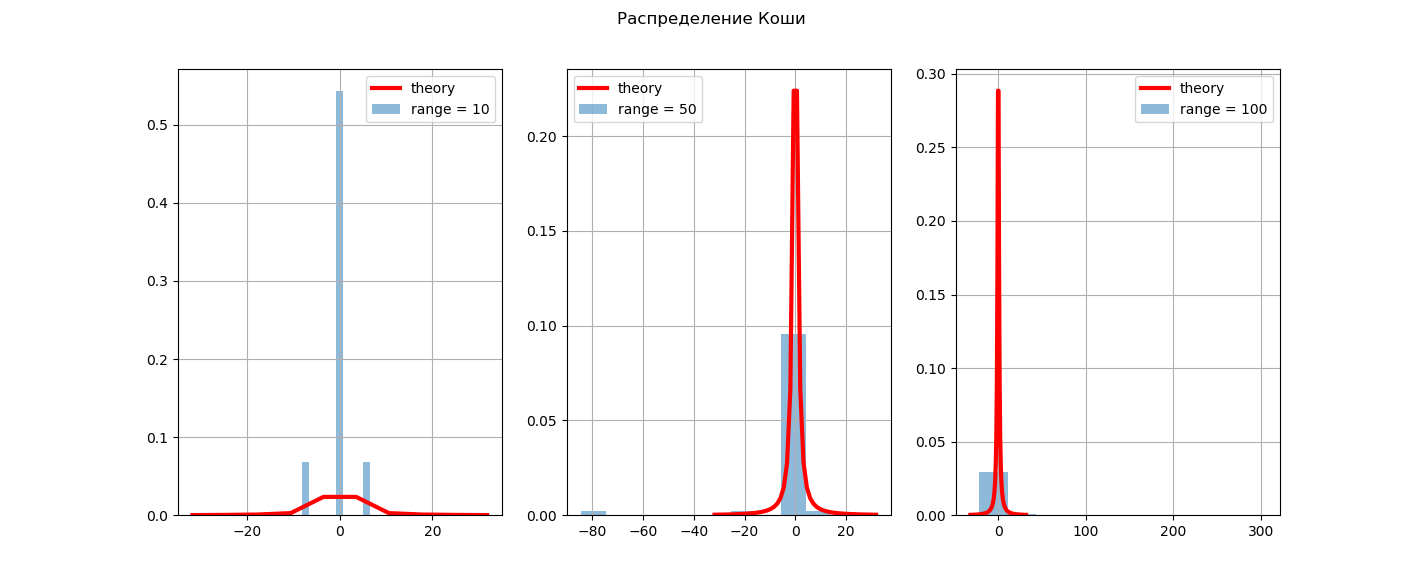
\includegraphics[width=\textwidth]{caushi.png}
\begin{center}
Рис. 2. 
\end{center}

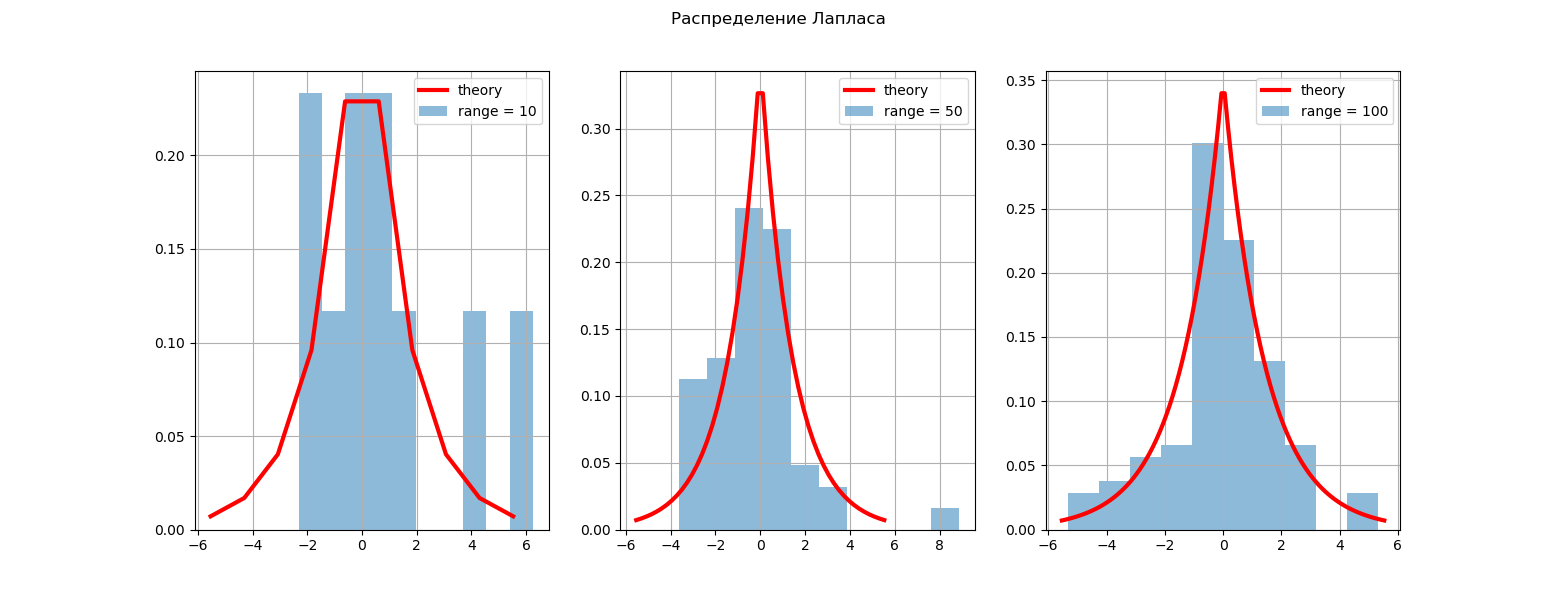
\includegraphics[width=\textwidth]{laplace.png}
\begin{center}
Рис. 3. 
\end{center}

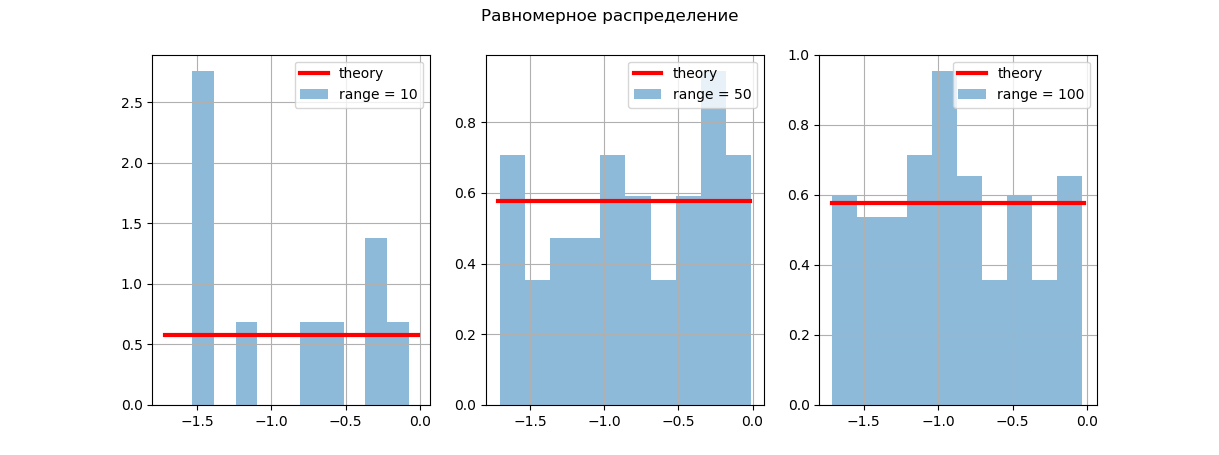
\includegraphics[width=\textwidth]{uniform.png}
\begin{center}
Рис. 4. 
\end{center}

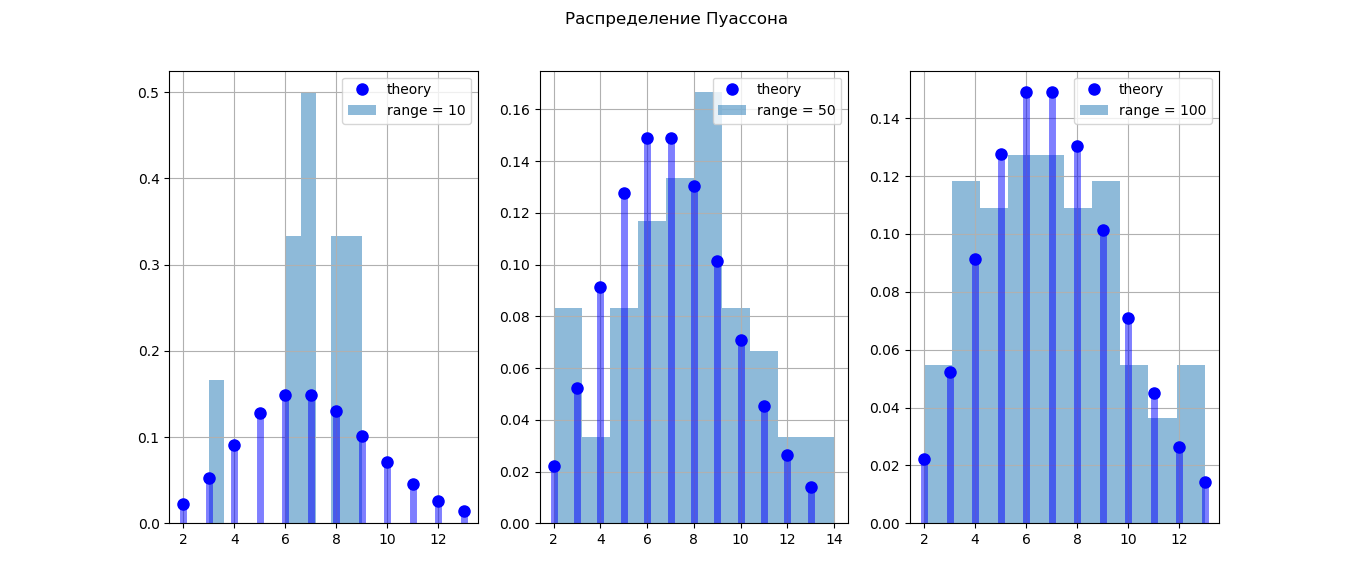
\includegraphics[width=\textwidth]{poisson.png}
\begin{center}
Рис. 5. 
\end{center}


\section{Обсуждение}

\subsection{Выводы}
В результате работы были построены графики для трёх выборок разных мощностей для каждого из рассматриваемых распределений. Из графиков видно, что с увеличением мощности выборки, диаграмма всё менее отклоняется от теоретического значения. Это иллюстрирует факт того, что при стремлении можности выборки к бесконечности диаграмма выборки будет оцениваться теоретической кривой с любой интересующей нас точностью.
\par
Конечно, за счёт того что размеры выборок довольно малы, то могут наблюдаться некоторые "выбросы" в конкретных точках (особенно заметно на самых левых графиках для мощности 10). Это объясняется тем, что значения выборки генерируются случайным образом и данных на такой мощности для построения теоретических оценок оказывается недостаточно.


\section{Литература}
\begin{enumerate}
\item Конспекты
\item Википедия
\end{enumerate}

\end{document}